\setauthor{Jonas Dorfinger}
Webmap ist als Webanwendung konzeptioniert, deshalb ist es wichtig für das Frontend eine Technologie zu wählen, welche
nicht nur langlebig ist, sondern auch eine gute Übersicht bietet.
Das beinhaltet unter anderem, dass eine große Community hinter dem Framework oder der Library steht,
aber auch die Anforderungen des Auftraggebers dürfen nicht unbeachtet bleiben.
Anhand dieser definierten Kriterien wurden die in 2021 beliebtesten Frameworks beziehungsweise Libraries verglichen und für eines entschieden.

\subsection{Framework vs. Library}
\label{subsec:framework-versus-library}
\setauthor{Jonas Dorfinger}
Sowohl Frameworks als auch Libraries sind Codes, welche oft auftretende Probleme einfach lösen sollen.
Um das konkret zu veranschaulichen, kann man dies mit einer Metapher besser beschreiben.

Eine Library ist wie der Besuch in einem Möbelhaus, man hat zwar grundsätzlich ein Haus aber keine Einrichtung, man
braucht also eine leichte Lösung um das Haus zu möblieren.
Einen Tisch selbst zu zimmern wäre zu aufwendig, deswegen wählt man einen Tisch aus der großen Auswahl in dem besuchten Geschäft.

Das Verwenden eines Frameworks ist wie der Bau eines Hauses, man hat ein paar Blaupausen und Vorgaben zum Design und zur
Architektur des neuen Gebäudes.
Man bekommt ein Grundgerüst zur Verfügung gestellt und darin kann man den Regelkonform frei agieren.

Zusammengefasst sind Frameworks Gerüste, welche durch Entwickler projektspezifisch erweitert werden müssen und Libraries
fertige Pakete, mit denen Programmierer Anwendungen um spezielle Funktionen erweitern.

\subsection{Angular}
\label{subsec:angular}
\setauthor{Jonas Dorfinger}
Angular wurde 2016 von Google ins Leben gerufen, seitdem ist es ein beliebtes Framework für die Webentwicklung.
Nur auf TypeScript basierend füllt es die Lücke zwischen der wachsenden Nachfrage von Technologien und traditionellen
Ideen zur Performance Optimierung.
Die Entwicklerplattform bietet etliche Services und Features an, dazu gehören nicht nur der Cross-Platform Support,
sondern auch eine built-in Geschwindigkeits- und Performanceoptimierung.
Auch für Unternehmen mit sehr hohen Nutzerzahlen ist Angular ein gern gewähltes Tool.
Ein großer Vorteil von Angular ist zudem, dass Angular unter einer Open-Source-Lizenz veröffentlicht
ist und somit nicht von dem Angular-Google Team, sondern auch von der Community betreut und erweitert wird.
Angular hat mit dem Two-Way-Binding einen großen Vorteil gegenüber React~\ref{subsec:react}.
Dieses Feature stellt sicher, dass die View und das Model in Echtzeit miteinander synchronisiert werden.
Das bedeutet, dass eine Änderung im Model direkt in der View angezeigt wird und umgekehrt auch.
~\cite{angular-features,what-is-angular}

\paragraph{Vorteile}
\begin{itemize}
    \item Features und Funktionalität wie das Two-Way-Binding sind direkt inkludiert
    \item Direkt eingebaute Features zum Updaten der View oder des Models.
    \item Komfortable Wiederverwendung von Components durch Dependency Injection
    \item Große Community zum Lernen und zur Fehlersuche
\end{itemize}

\paragraph{Nachteile}
\begin{itemize}
    \item Schwieriger zu lernen, da Angular so groß ist und es viele mögliche Lösungen gibt
    \item Durch die riesigen und komplexen Strukturen kann es sein, dass bei großen dynamischen Applikationen Performance Probleme auftreten
    \item Angular ist ein full-package Framework, weshalb es für kleine Applikationen ungeeignet ist
\end{itemize}

\subsection{React}
\label{subsec:react}
\setauthor{Jonas Dorfinger}
ReactJS ist die größte Konkurrenz von Angular, mit einem Vielfachen an Marktanteilen.
Im Gegensatz zu Angular wird React von Facebook gewartet und betreut und verfügt über die Funktionalität des virtuellen
Document Object Models (DOM).
Das virtuelle DOM verbessert die Performance und verringert die Dauer von Render Prozessen, da nur die Inhalte verwendet werden,
welche sich auch tatsächlich verändert haben und nicht die gesamte View neu gerendert wird.
Durch dieses Feature wird eine Plattform geschaffen, welche sich sehr gut für Applikationen mit großem Traffic eignet.
Ein Alleinstellungsmerkmal ist dazu auch noch, dass React Server-Side Rendering unterstützt.
Für SPAs, also Single Page Applications ist es empfehlenswert sich für React zu entscheiden, durch das Wiederverwenden der
Komponenten kann man in kurzer Zeit gute und interaktive User Interfaces entwickeln.

\begin{figure}[hbt!]
    \centering
    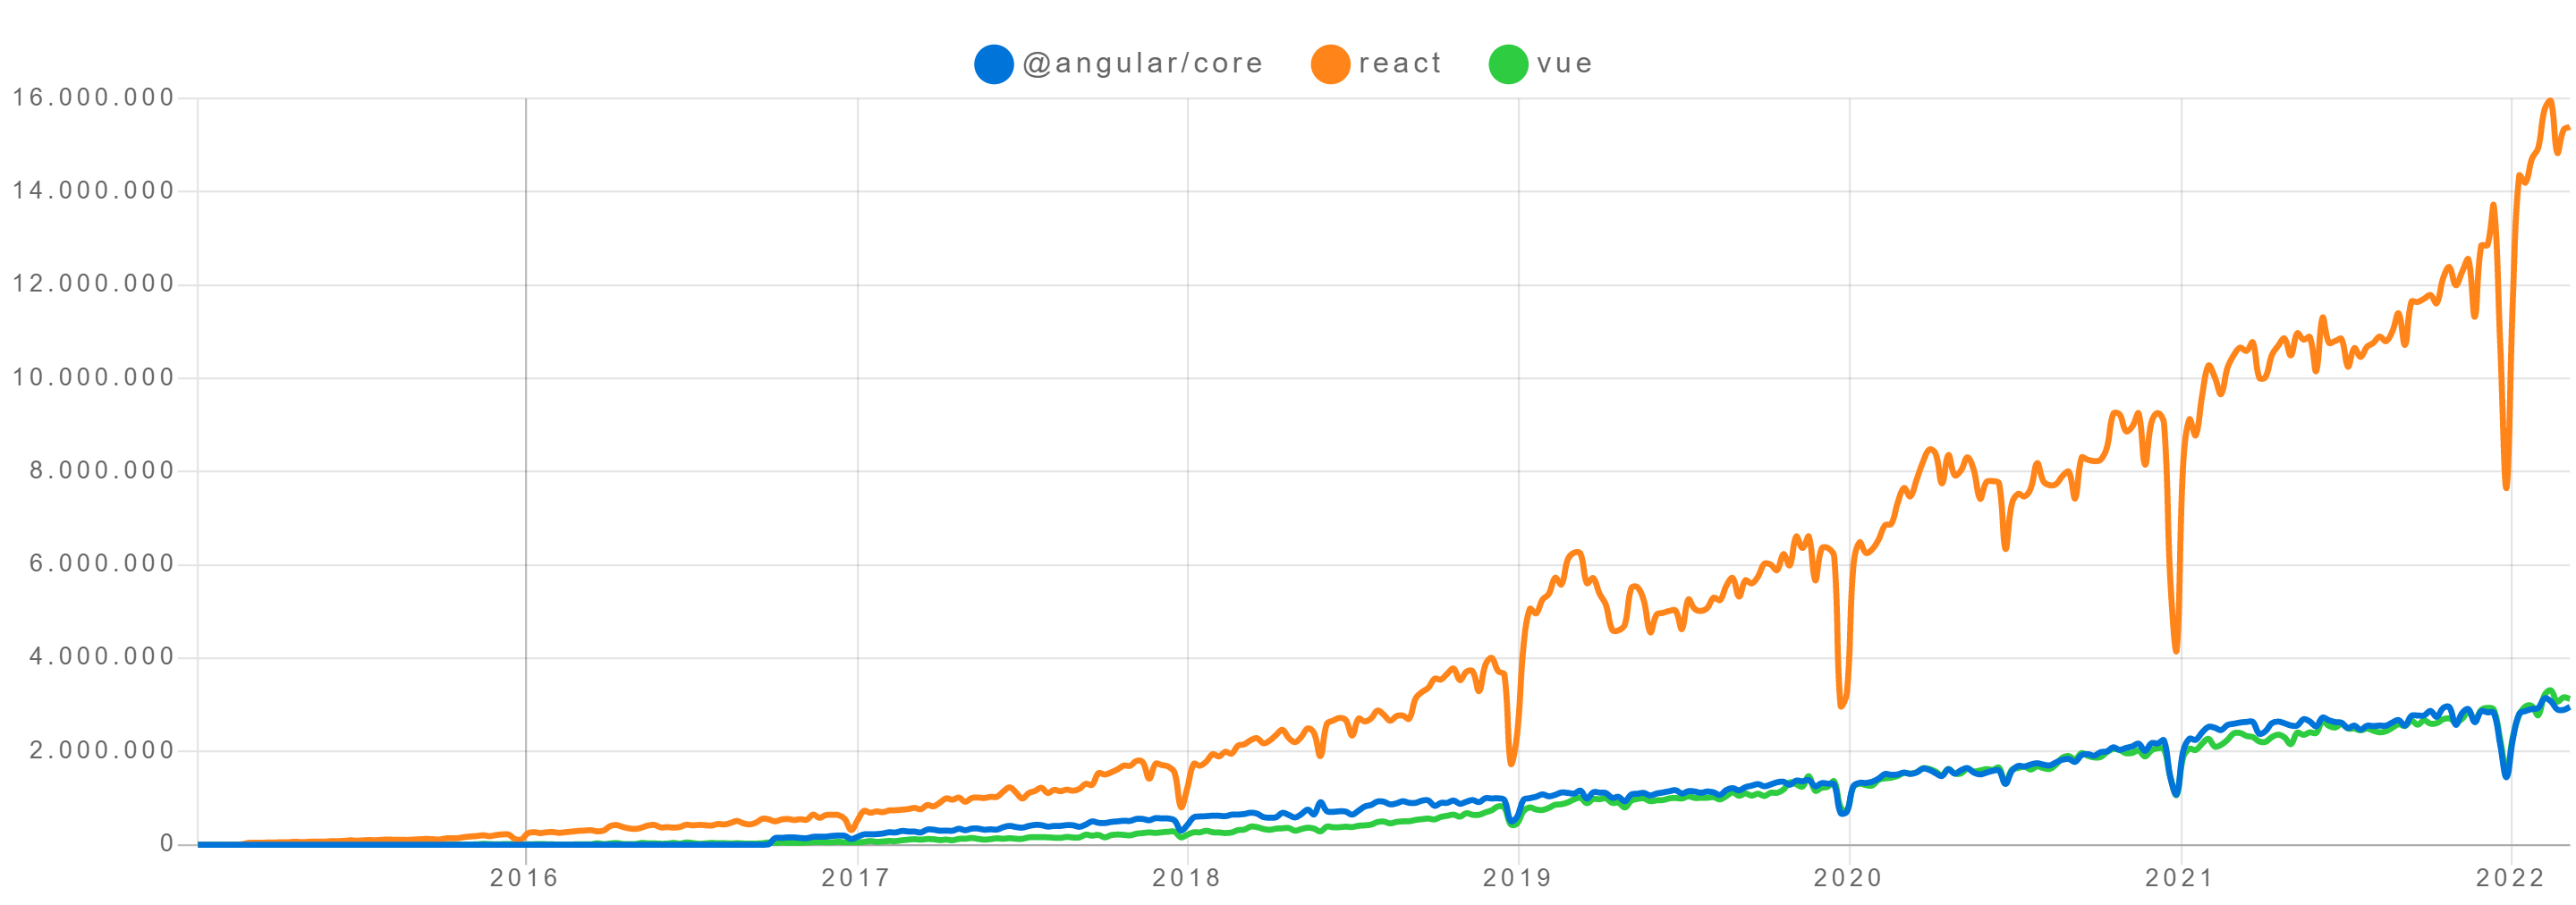
\includegraphics[scale=0.15]{pics/angular-react-vue-npm-chart}
    \caption{wöchentliche Downloads~\cite{angular-react-vue-stats}}
    \label{fig:angular-react-vue-chart}
\end{figure}
\begin{figure}[hbt!]
    \centering
    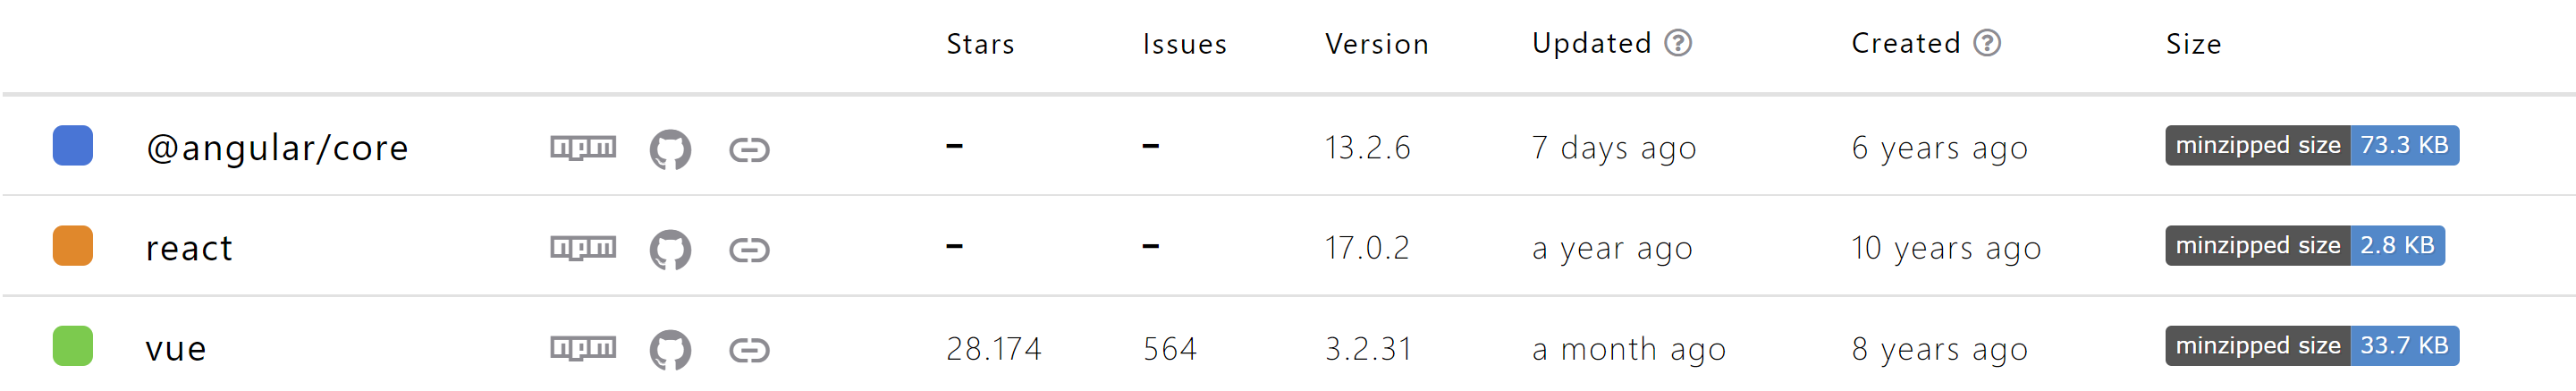
\includegraphics[scale=0.5]{pics/angular-react-vue-npm-stats}
    \caption{Direkter Vergleich der Frameworks~\cite{angular-react-vue-stats}}
    \label{fig:angular-react-vue-stats}
\end{figure}

\paragraph{Vorteile}
\begin{itemize}
    \item Durch das virtuelle DOM ist die Performance sehr optimiert und kann gut mit vielen gleichzeitigen Zugriffen zurechtkommen
    \item Unabhängige Components sind leicht zu implementieren und zu wiederverwenden
    \item React Developer Tools sind sehr ausgereift mit einer großen Nutzbarkeit
\end{itemize}

\paragraph{Nachteile}
\begin{itemize}
    \item Durch etliche Updates ist die Dokumentation lückenhaft
    \item Schnelle Änderungen in kurzer Zeit, neu gelerntes ist in naher Zukunft bereits wieder "alt"
    \item Inhalte wie JSX sind komplex und schwer zu lernen
    \item ReactJS setzt einiges an Erfahrung in JavaScript oder TypeScript voraus
\end{itemize}

\subsection{Vue}
\label{subsec:vue}
\setauthor{Jonas Dorfinger}
Vue.js ist ein kleines, aber sehr einfach funktionierendes Frontend System und wird immer beliebter.
Es ist gut sehr darin, Probleme mit denen Angular Developer umgehen müssen zu vermindern oder gar zu lösen.
Vue.JS ist außerdem sehr leichtgewichtig und klein, hat aber trotzdem viele nützlich Features wie das Two-Way-Binding
out-of-the-box dabei, auch die Verwendung als PWA (Progressive Web Apps) ist möglich.
Der wohl größte Nachteil ist die niedrige Trucknumber~\cite{truck-factor-of-popular-github-projects, what-is-the-bus-factor}.
Die Trucknumber bei Projekten beschreibt, wie viele Personen ausfallen müssen, dass das Projekt weiterlaufen kann.
Je höher die Trucknumber, desto mehr Personen könnten ausfallen und das Projekt würde also weiterlaufen.
Im Gegensatz dazu, je kleiner die Trucknumber, desto weniger Personen können ausfallen, das geht so weit, dass das gesamte
Projekt an einer einzigen Person hängt.
Das letzte Beispiel ist fast bei Vue.js gegeben, in das Core Repository von Vue committed regelmäßig nur der Gründer
von Vue, Evan You.
VueJS kann in beiden, TypeScript und JavaScript geschrieben werden.

\paragraph{Vorteile}
\begin{itemize}
    \item Sehr leicht zu lernen, vor allem mit basis JavaScript Wissen
    \item Flexibles App Layout
    \item Umfangreiche und ausführliche Dokumentation
\end{itemize}

\paragraph{Nachteile}
\begin{itemize}
    \item Sehr kleine Community (Wartung und Support)
    \item Sehr geringe Truck Number
    \item Stabilitätsprobleme bei großen Projekten
\end{itemize}

\begin{figure}[hbt!]
    \centering
    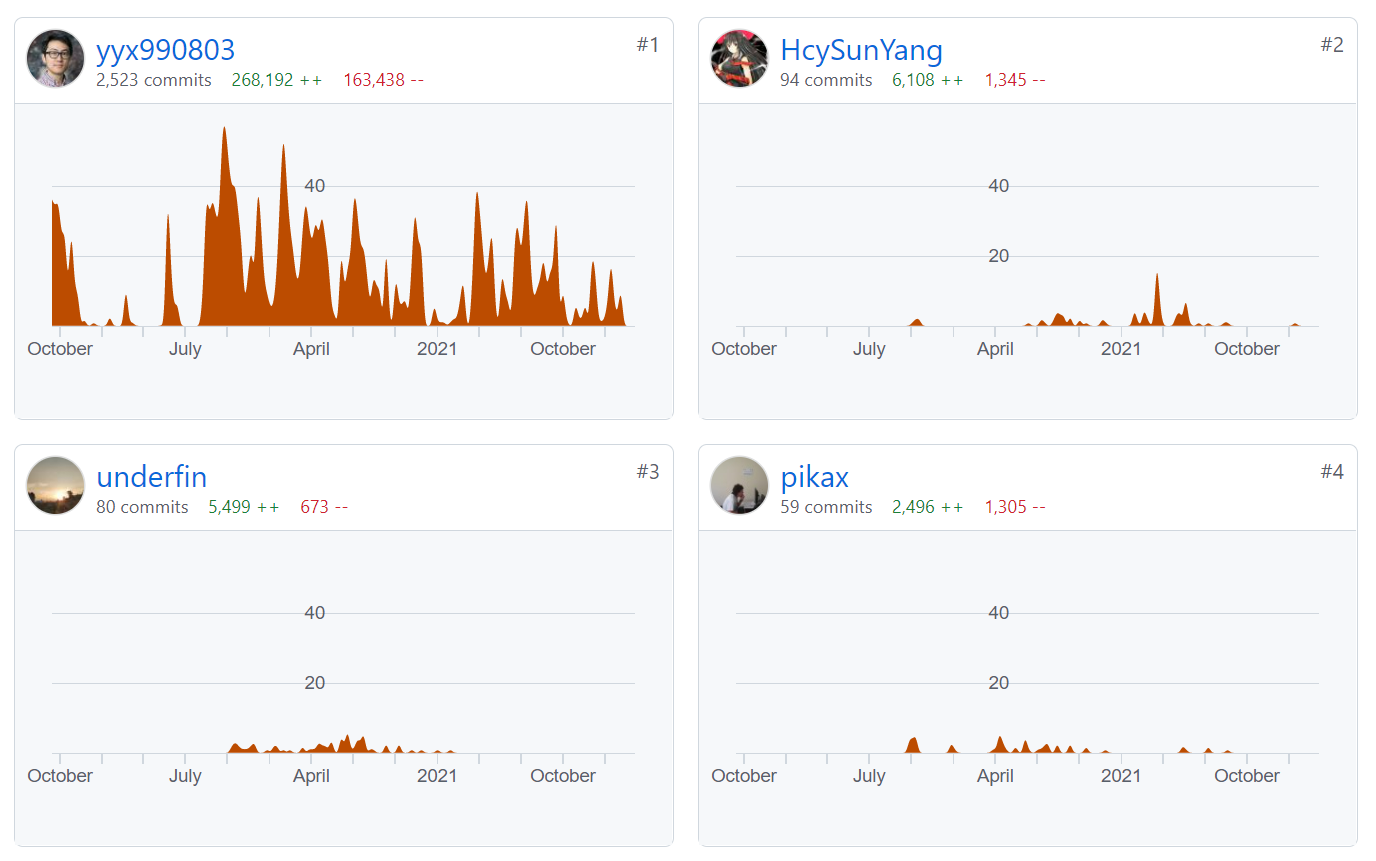
\includegraphics[scale=0.8]{pics/vue_contributions}
    \caption{Vue.js Core Repository Commits im Zeitraum 16. September 2018 - 9. Februar 2022~\cite{VueJSContribution}}
    \label{fig:vue_contributions}
\end{figure}

~\cite{best-frontend-frameworks, best-frontend-framework-2022, angular-vs-react-vs-vue}

\subsection{Verwendung von Angular}
\setauthor{Jonas Dorfinger}

\subsubsection{Warum Angular?}
\setauthor{Jonas Dorfinger}
Einer der Entwickler hat bereits mehr als zweieinhalb Jahre Erfahrung in der Entwicklung von UserInterfaces und Web-Oberflächen mit Angular.
Zusätzlich dazu wird Angular in der HTL Leonding ab dem 4. Jahrgang in der Abteilung Medientechnik unterrichtet, wodurch
die Wahl auf Angular naheliegend war.
Unabhängig von der Schule und den Entwicklern ist es außerdem eine Anforderung der Betreuerfirma triply Angular zu verwenden,
weil triply bei allen Frontend Projekten auf Angular vertraut und um diese Konsistenz zu bewahren ist Angular die logische Wahl.

\subsubsection{Angular installieren und verwenden}
\setauthor{Jonas Dorfinger}

\paragraph{Node.js}
\label{Node.js}
Node.js ist eine asynchrone open-source Event gesteuerte JavaScript Entwicklerumgebung.
Node.js ist Plattformunabhängig, das heißt, dass in node geschriebene Anwendungen sowohl auf Windows oder Linux als auch auf macOS problemlos funktionieren.
JavaScript wird grundsätzlich im Browser ausgeführt, durch node kann JavaScript jedoch auch serverseitig ausgeführt werden.
Dabei erhält man durch die Node.js API umfangreiche Funktionen, um mit dem lokalen Betriebssystem zu interagieren.
Node.js wird verwendet, um skalierbare Netzwerk Applikationen zu designen.
Im folgenden Beispiel wird gezeigt, wie man einen einfachen Node.js Webserver implementiert.
Durch diese Implementierung können etliche Verbindungen gleichzeitig behandelt werden.
Bei jeder Verbindung wird die Callback Funktion ausgeführt.
Werden keine Verbindungen aufgebaut, so geht Node.js in den Wartezustand.
Wenn man Node.js verwendet, muss man sich keine Sorgen über dead-locks machen, weil es durch die Asynchronität keine locks gibt.
Node.js Funktionen führen kaum I/O Prozesse durch,
dadurch kann ein Prozess nie blockieren außer es wird die I/O Funktion synchron über die Node.js Library aufgerufen.
Weil keine Prozesse blockieren, ist es naheliegend skalierende Systeme in Node.js zu entwickeln~\cite{about-node-js}.

\begin{lstlisting}[label={lst:hello-world.js}]{hello-world.js}
const http = require('http');

const hostname = '127.0.0.1';
const port = 3000;

const server = http.createServer((req, res) => {
  res.statusCode = 200;
  res.setHeader('Content-Type', 'text/plain');
  res.end('Hello World');
});

server.listen(port, hostname, () => {
  console.log(`Server running at http://${hostname}:${port}/`);
});
\end{lstlisting}

\paragraph{npm}
npm oder auch ausgeschrieben der Node-Package-Manager ist eine Software um Packages zu Node.js Applikationen hinzuzufügen.
npm wird standardmäßig mit Node.js mitinstalliert, es handelt sich um eine CLI (Command-Line-Interface) welche auf die online registry zugreift.
Die npm-registry ist eine Online-Datenbank welche public (open-source) und private (auch kostenpflichtige) Packages zur Verfügung stellt.
Die Packages werden über die CLI installiert und können über die \href{https://npmjs.com}{npm Website} gesucht werden.
npm ist ein Produkt von Github, Github wiederum gehört seit 2018 zu Microsoft~\cite{microsoft-acquires-github}.

\paragraph{TypeScript}
\label{TypeScript}
TypeScript ist eine typisierte Programmiersprache welche auf JavaScript aufbaut.
TypeScript ist außerdem eine Übermenge von JavaScript.
Das bedeutet, dass TypeScript alle Eigenschaften von JavaScript hat und aber noch eigene Funktionalität mitbringt.
Folgende Features werden im Gegensatz zu JavaScript unterstützt:

\begin{itemize}
    \item Typisierung von Variablen (auch während des Kompilierens)
    \item Type inference
    \item Type erasure
    \item Interfaces
    \item Enumerated types
    \item Generics
    \item Namespaces
    \item Tuples
    \item Async/await
    \item Classes
    \item Modules
    \item Verkürzte Syntax von anonymen arrow-functions
    \item Optionale Parameter and Defaultwerte für Parameter
\end{itemize}

Wenn man ein TypeScript Programm ausführt, dann wird der Quellcode von TypeScript Code in JavaScript Code transpiled.
Dies wird erzielt, indem eine von mehreren möglichen Optionen ausgewählt wird.
Die Auswahl beschränkt sich dennoch auf den TypeScript Checker oder Babel, beide Varianten sind stark verbreitet.
TypeScript kann sowohl Clientseitig, als auch Serverseitig (zum Beispiel in Kombination mit Node.js) eingesetzt werden.

\paragraph{Beispiel: Funktionen mit und ohne Types} \

JavaScript Funktion zum Addieren von 2 Zahlen (ohne types)
\begin{lstlisting}[label={lst:add-function-js}]{app.js}
function add(number1, number2) {
    return number1 + number2;
}


add(6, 9);  // returns 15

add("Hallo ", "Welt");  // returns "Hallo Welt"
\end{lstlisting}

Bei JavaScript gibts es keine typisierten Funktionen, deshalb verhält sich die Funktion immer den Parametern entsprechend.

\

TypeScript Funktion zum Addieren von 2 Zahlen (mit types)
\begin{lstlisting}[label={lst:add-function-ts}]{app.ts}
function add(number1: number, number2: number): number {
    return number1 + number2;
}

add(6, 9);  // returns 15

add("Hallo ", "Welt");  // Error: Argument of type 'string' is not assignable to parameter of type 'number'.
\end{lstlisting}

Da TypeScript Typisierungen unterstützt, wird bereits zur Compilezeit sichergestellt, dass die richtigen Daten als Parameter übergeben werden.
Deshalb tritt beim zweiten Aufruf ein Error auf, weil ein String nicht als Nummer verwendbar ist.

\cite{typescript-landing-page, what-is-typescript}

\subsubsection{Wie funktioniert Angular?}
\setauthor{Jonas Dorfinger}
\emph{Ivy} ist die neue Compilation und Rendering Pipeline für Angular.
Seit der Angular Version 9 wird standardmäßig die neue Pipeline verwendet und ersetzt damit die Alter Pipeline,
welche unter dem Namen \emph{View Engine} bekannt ist.

Da \emph{Ivy} nicht nur eine Rendering Engine, sondern auch eine Compile Engine ist, öffnen sich ganz neue Türen was die
Optimierung für und über das gesamte Framework angeht.

Anstatt Template Daten zu generieren, diese in einen Interpreter zu geben, der wiederrum entscheidet, welche Operationen
ausgeführt werden, wird direkt eine Sammlung an \emph{Template Instructions} generiert.
Die \emph{Template Instructions} beinhalten die Logik, welche Components instanziiert, DOM Nodes erstellt und Change Detection in Echtzeit ausführt.

\begin{figure}[hbt!]
    \centering
    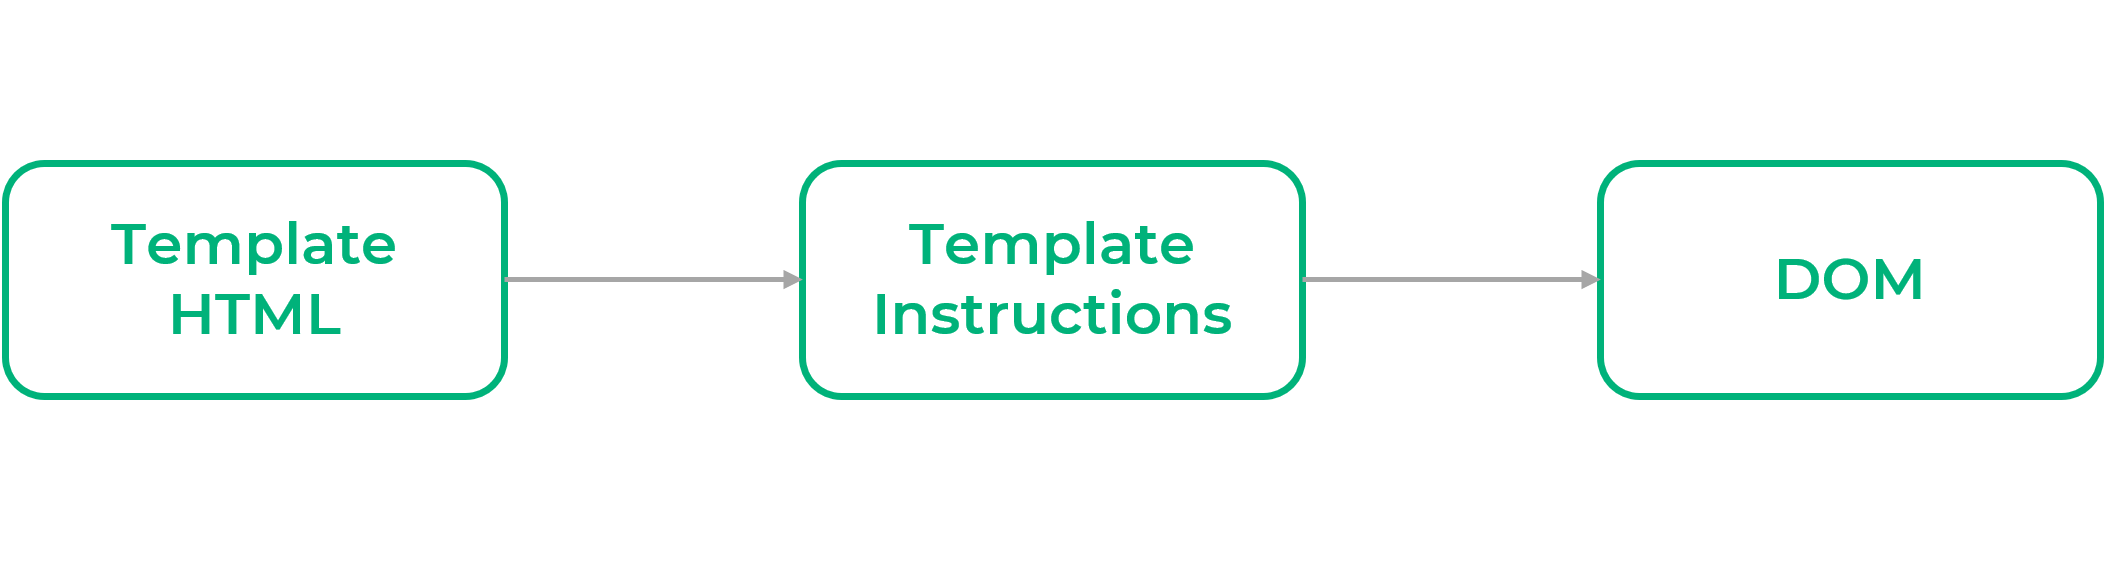
\includegraphics[scale=.4]{pics/ivy-pipeline}
    \caption{Ivy Pipeline}
    \label{fig:ivy-pipeline}
\end{figure}

\paragraph{Incremental DOM}
Jede Component wird in eine eigene Sammlung an Instructions compiled, diese erstellen DOM Trees und aktualisieren die
Daten an Ort und Stelle, wenn diese sich ändern.
Zum Erstellen des \emph{Document Object Models} gibt es drei verschieden Funktionen:

\begin{itemize}
    \item \emph{elementStart} (opening tag)
    \item \emph{text} (inner html)
    \item \emph{elementEnd} (closing tag)
\end{itemize}

Beim Aktualisieren des DOMs wird nicht automatisch jedes Mal ein komplett neuer Tree erstellt, sondern es werden alle
Nodes verglichen und nur jene verändert, welche auch tatsächlich verändert wurden.
Das spart nicht nur Arbeitsspeicher, sondern auch Zeit.

Der Grund warum Incremental DOM verwendet sind die Ziele welche erreicht werden möchten.
Der Fokus liegt auf einer besseren Performance von Web-Applikationen auf Mobilen Endgeräten (Handys, Tablets).
Um dies zu erreichen, ist es erforderlich zwei Dinge zu optimieren, \emph{bundle size} und \emph{memory footprint}.


\paragraph{Shakable Tree}
Bei Verwendung der Incremental DOM Strategie wird nicht die Component interpretiert, sondern jede Component verweist auf
verschiedene Instructions.
Wenn kein Verweis auf eine Instruction zu finden ist, dann wird dieser Teil nicht verwendet und ist somit überflüssig.
Durch die Vorteile von Incremental DOM ist dies bereits zur Compile Zeit bekannt, weshalb alle nicht benützten Instructions
vom bundle entfernt, was wiederrum die \emph{bundle size} beträchtlich verringern kann.

\begin{figure}[hbt!]
    \centering
    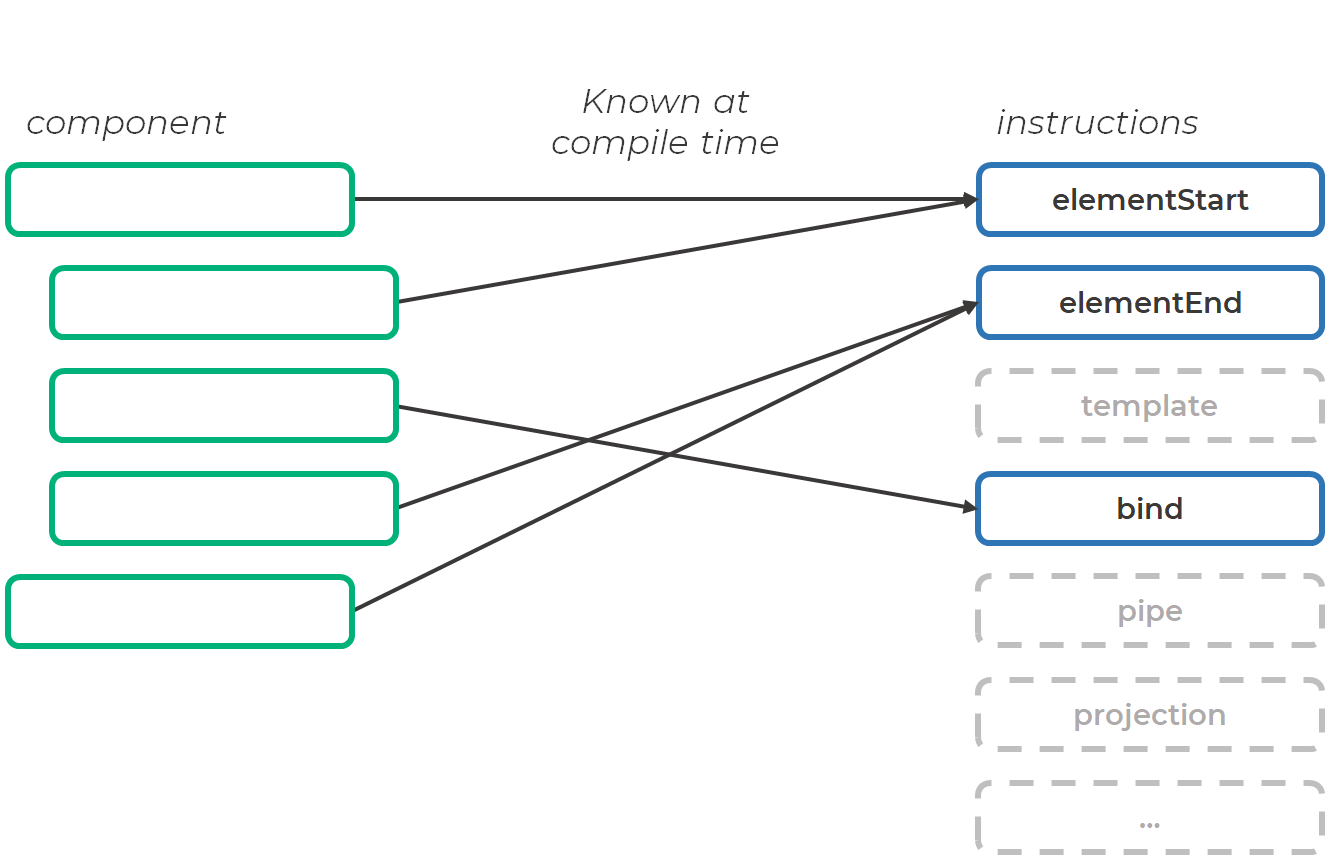
\includegraphics[scale=.6]{pics/shakable-tree}
    \caption{Skakable Tree}
    \label{fig:shakable-tree}
\end{figure}

\cite{rendering-engine-ivy, incremental-dom}

\cleardoublepage

\subsubsection{Angular Material}
\setauthor{Jonas Dorfinger}
Angular Material ist eine Component-Library von Angular, diese beinhaltet stylistisch aufeinander abgestimmte Elemente.
Diese Komponenten können ganz einfach importiert werden, durch das Responsive Design der Inhalte, eignen sich diese sehr gut
für die Umsetzung einer Web-Oberfläche, da nicht viel Zeit für das Design verloren geht, sondern der Fokus voll und ganz
auf die Funktionalität gelegt werden kann.

Angular Material kann jederzeit über einen Konsolenbefehl zu einem Angular Projekt hinzugefügt werden:
\begin{center}
    \centering{ng add @angular/material}
\end{center}

Bei der Installation kann man bereits vordefinierte Themes von Angular auswählen, zur Auswahl stehen insgesamt 4 verschiedene,
zwei Dark- und zwei Lighttheme Varianten~\cite{angular-material-predefined-themes}:

\begin{itemize}
    \item Deep Purple \& Amber (Light)
    \item Indigo \& Pink (Light)
    \item Pink \& Blue-grey (Dark)
    \item Purple \& Green (Dark)
\end{itemize}

Weiters hat man die Möglichkeit eigene Themes zu erstellen.
Mithilfe von Custom Themes können die von Angular bereitgestellten Komponenten für jedes Projekt individuell eingefärbt werden.
Um das zu erreichen, wählt man beim Installieren die fünfte Auswahlmöglichkeit \emph{Custom} aus.
Dies erstellt, den dafür benötigten Code in dem \emph{styles.scss} File.
Man kann sich über diverse Internet Seiten Farbpaletten generieren lassen, diese werden benötigt, um ein eigenes Theme zu gestalten.
Ein Angular Theme hat genau "drei" verschieden Farben, wobei es eher Farbpaletten sind.

\paragraph{primary-palette}
Die Primary Palette legt die Hauptfarbe fest, welche in fast allen Komponenten standardmäßig verwendet wird.
Man kann allerdings auch bei den meisten Komponenten individuell als Parameter angeben, welche der drei Paletten verwendet werden soll.

\paragraph{accent-palette}
Die Accent Palette definiert eine Akzentfarbe, welche einen hohen Kontrast zur Hauptfarbe haben soll, um bestimmte Elemente
besser hervorheben zu können.

\paragraph{warn-palette}
Die Warn Palette besteht meist aus einem Rot, welcher für Fehlermeldungen verwendet wird.

\linebreak
\linebreak
\linebreak

Eine Farbpalette besteht aus einer Basisfarbe und mehrere abstufungen dieser Farbe, um auch hier unterschiedliche Töne für
Hervorhebungen zu haben.

Ein Beispiel einer Farbpalette für eine primary-palette:

\begin{lstlisting}[label={lst:custom-primary-color-palette}]{style.scss}
$primary-palette: (
  50 : #e2f3f4,
  100 : #b8e2e4,
  200 : #88ced2,
  300 : #58babf,
  400 : #35acb2,
  500 : #119da4,
  600 : #0f959c,
  700 : #0c8b92,
  800 : #0a8189,
  900 : #056f78,
  A100 : #a7f7ff,
  A200 : #74f3ff,
  A400 : #41efff,
  A700 : #27ecff,
  contrast: (
    50 : #000000,
    100 : #000000,
    200 : #000000,
    300 : #000000,
    400 : #000000,
    500 : #ffffff,
    600 : #ffffff,
    700 : #ffffff,
    800 : #ffffff,
    900 : #ffffff,
    A100 : #000000,
    A200 : #000000,
    A400 : #000000,
    A700 : #000000,
  )
);
\end{lstlisting}

Insgesamt hat man die Auswahl aus 36 verschiedenen Komponenten~\cite{angular-material-component-overview,angular-material-description,angular-material-with-angular}.

Die Komponenten werden ganz einfach über einen Custom HTML Tag eingebunden.

\subsubsection{triply Material Library}
\setauthor{Jonas Dorfinger}
Triply hat in den letzten Monaten einige eigene Angular Komponenten erstellt und in einer internen Bibliothek
gesammelt, vor allem auf diese Inhalte wurde zurückgegriffen, um zum Beispiel einen Slider oder einen true/false Switch
zu verwenden.
Der Unterschied zu Angular Material liegt darin, dass die Firmeninterne Library aus Files besteht, welche in das Projekt
kopiert werden, vereinfach gesagt, man verwendet dabei Custom-Components.

\begin{figure}[hbt!]
    \centering
    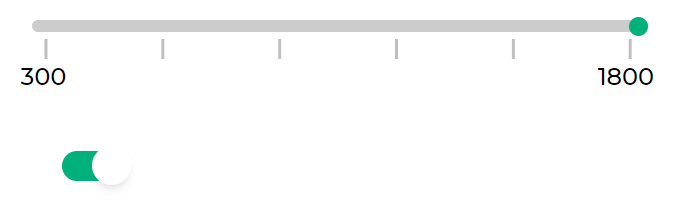
\includegraphics[scale=1]{pics/triply-material-library}
    \caption{Triply Slider und Triply Switch}
    \label{fig:triply-material-library}
\end{figure}

\subsubsection{Model-View-Controller Design Pattern}
\setauthor{Jonas Dorfinger}
Dieses Pattern wird oft für die Entwicklung von User Interfaces verwendet,
dabei wird die Logik in drei verschiedenen Elementen (Files) aufgeteilt.
Das wird gemacht, um interne Abbildungen und Referenzen von Daten beziehungsweise Informationen
in einer Art und Weise aufzuteilen.
Das Model ist von der restlichen Anwendung komplett
unabhängig.
Im Gegensatz dazu ist die View stark abhängig von der zu programmierenden Anwendung.
Die Aufgabe der View beschränkt sich rein auf die Visualisierung der durch den Controller bereitgestellten Daten.
Der Controller hat eine Vermittlerrolle zwischen Model und View.
In Angular ergeben alle drei Files eine gemeinsame Component.

\paragraph{Model}
Das Model File ist das Herzstück der Component, es beinhaltet alle Daten
Strukturen und den Aufbau, dabei werden Daten, Logik und Regeln
der Component festgelegt und verwaltet.
Bei Angular sind das entweder Interfaces oder Klassen ohne Logik.
~\cite{angular-design-patterns}

\paragraph{View}
Die View beinhaltet alle Details zur Darstellung der Daten und Informationen.
Es kann mehrere Views für die gleiche Information geben, zum Beispiel ein
Balkendiagramm für den Manager oder eine Tabelle für die Buchhaltung.

\paragraph{Controller}
Der Controller ist das Gehirn einer Component, er ist das Verbindungsstück zwischen View und Model.
Dabei werden die Daten mittels Getter-Funktionen aus dem Model geladen und so verändert beziehungsweise so manipuliert, sodass die View diese richtig
anzeigen kann.
Wenn Änderungen der Daten durch die gemacht werden, speichert der Controller diese Änderung mittels Setter-Funktionen im Model.

\begin{figure}[hbt!]
    \centering
    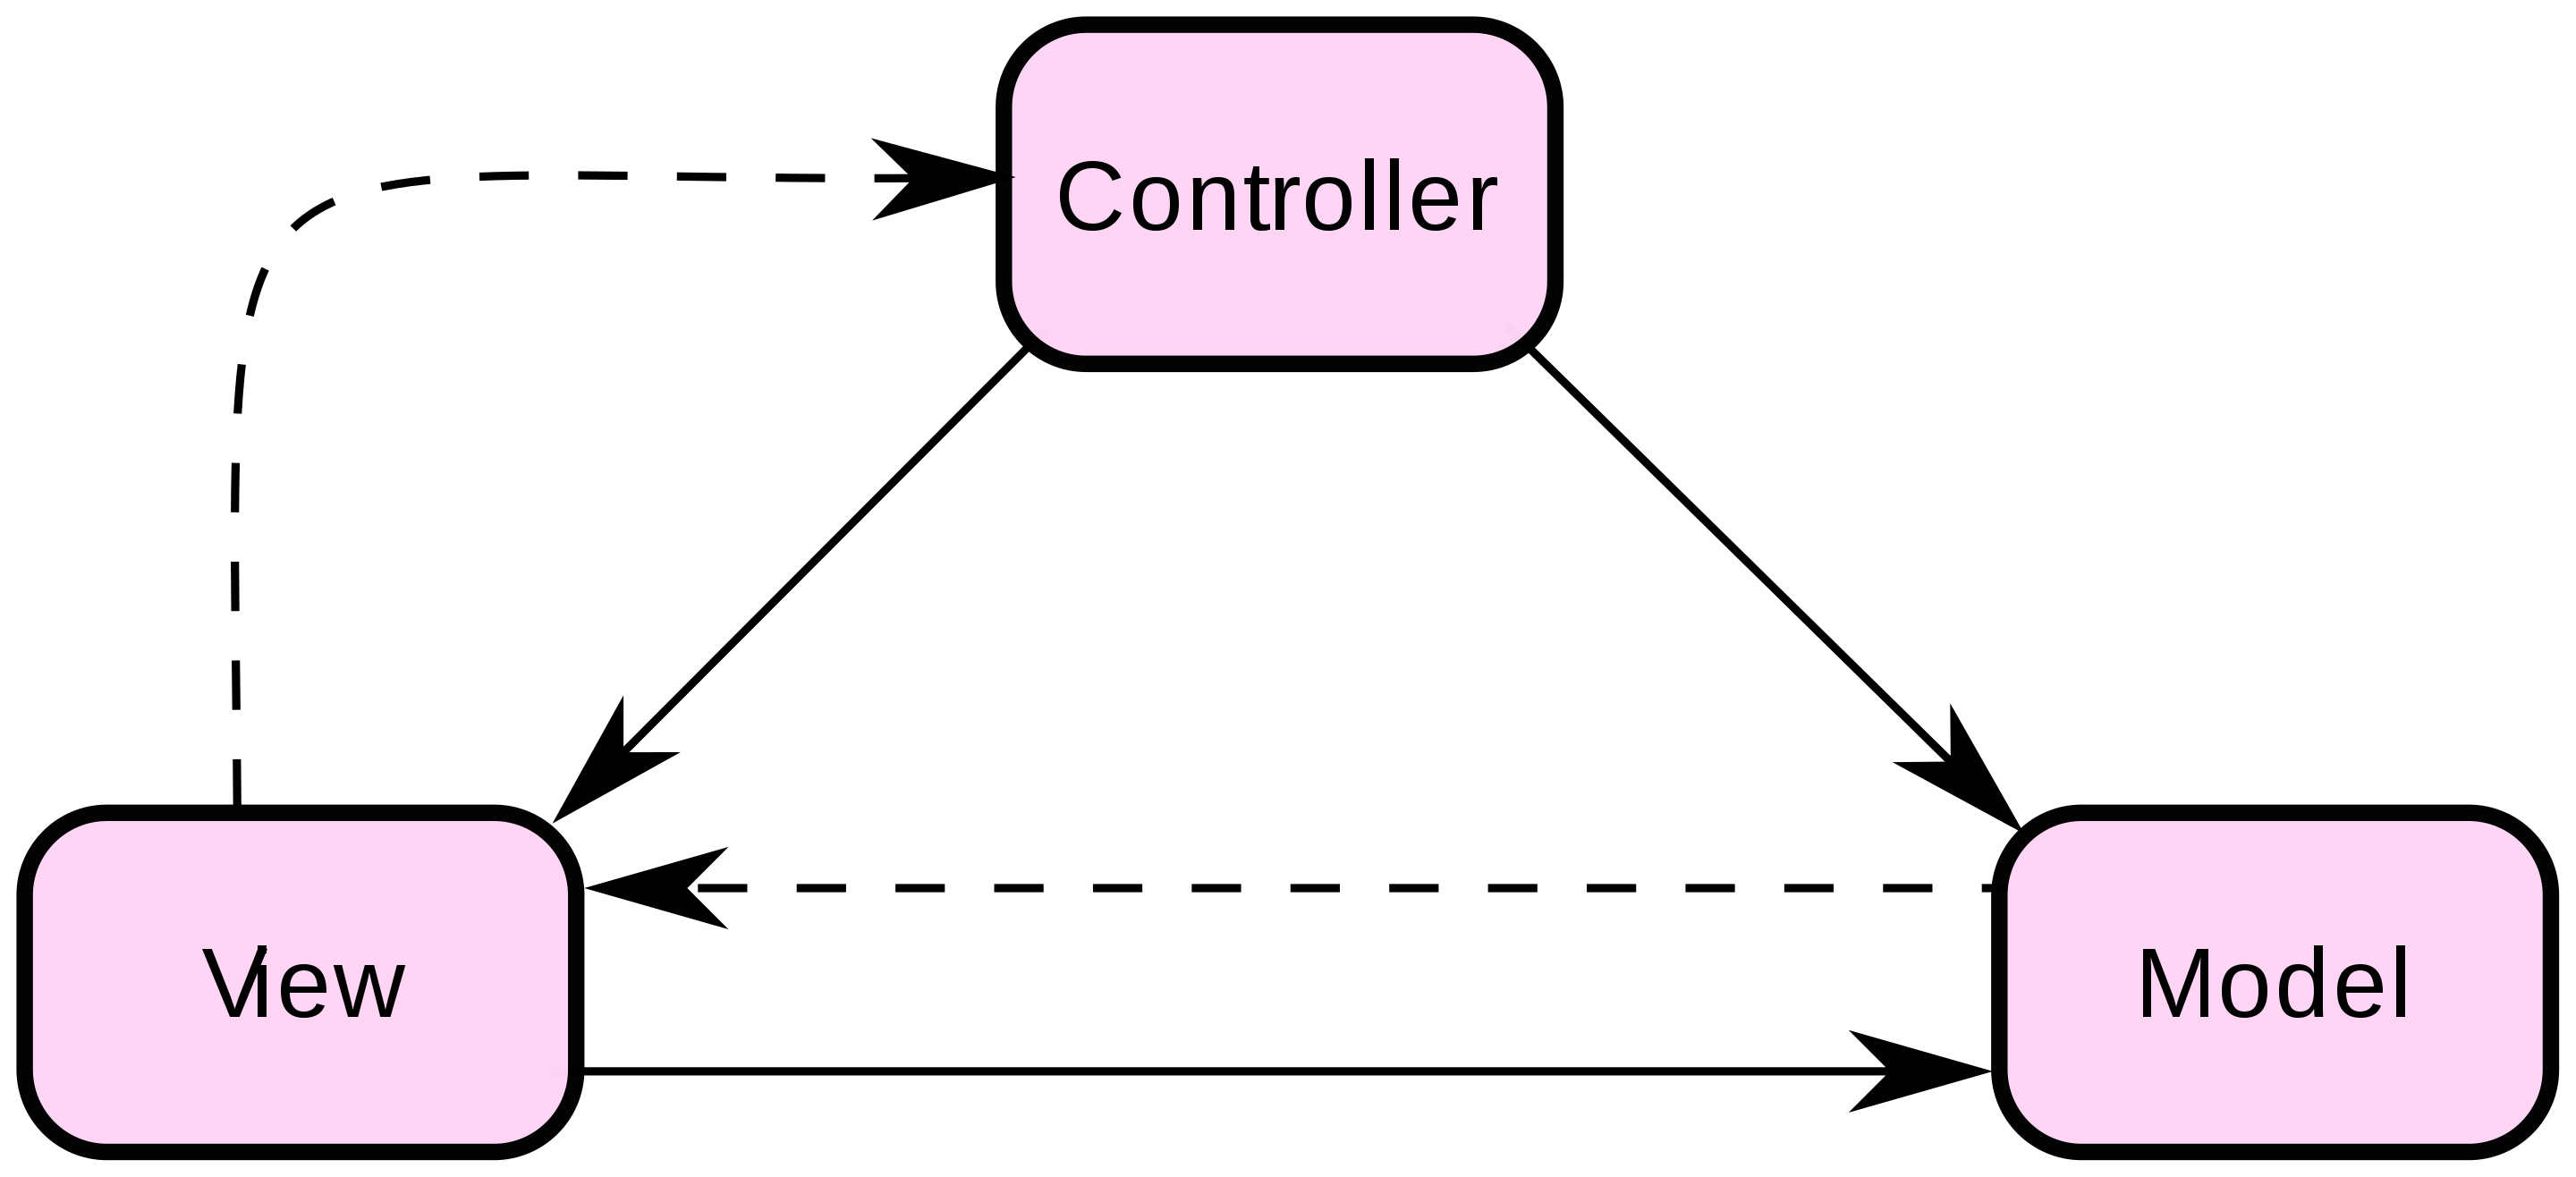
\includegraphics[scale=0.1]{pics/mvc_design_pattern}
    \caption{Model-View-Controller-Pattern}
    \label{fig:mvc_design_pattern}
\end{figure}
